\uuid{8eRQ}
\exo7id{7289}
\titre{exo7 7289}
\auteur{mourougane}
\organisation{exo7}
\datecreate{2021-08-10}
\isIndication{false}
\isCorrection{false}
\chapitre{Géométrie affine euclidienne}
\sousChapitre{Géométrie affine euclidienne du plan}
\module{Géométrie}
\niveau{L2}
\difficulte{}

\contenu{
\texte{
% cf. https://en.wikipedia.org/wiki/Napoleon%27s_problem
La question de trouver le centre d'un cercle à la règle et au compas a été 
étudiée à l'exercice~\ref{centre-regle-compas}. On étudie maintenant une 
construction au compas seul.

\begin{center}
    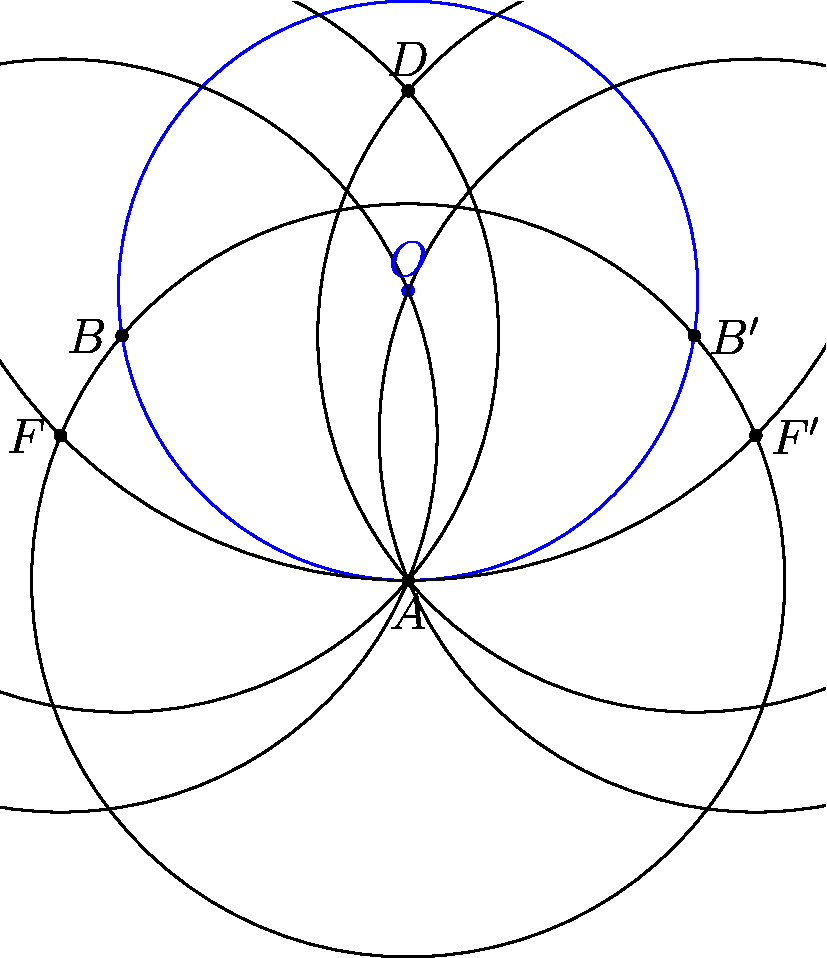
\includegraphics[scale=1]{images/img-mour-041}
\end{center}

% [[figure asymptote]]

%\begin{center}
%\begin{asy}
%size(7cm, 0);
%point O = (0, 0); dot("\(O\)", O, N, blue);
%circle C0 = circle(O, 1); draw(C0, blue);
%point A = (0, -1); dot("\(A\)", A, S);
%circle C1 = circle(A, 1.3); draw(C1);
%point[] B = intersectionpoints(C0, C1);
%dot("\(B\)", B[0], W); dot("\(B'\)", B[1], E);
%circle C2 = circle(B[0], abs(A - B[0])); clipdraw(C2);
%circle C3 = circle(B[1], abs(A - B[1])); clipdraw(C3);
%point[] AD = intersectionpoints(C2, C3);
%point D = (AD[0] == A) ? AD[1] : AD[0];
%dot("\(D\)", D, N);
%circle C4 = circle(D, abs(A - D)); clipdraw(C4);
%point[] F = intersectionpoints(C1, C4);
%dot("\(F\)", F[0], W); dot("\(F'\)", F[1], E);
%clipdraw(circle(F[0], abs(A - F[0])));
%clipdraw(circle(F[1], abs(A - F[1])));
%\end{asy}
%\end{center}

Soit \(\mathcal{C}\) un cercle (dont on ne connaît pas le centre). 
Soit \(A\) un point de \(\mathcal{C}\), et soit \(\mathcal{C}'\) 
un cercle de centre \(A\), qui coupe \(\mathcal{C}\) en deux points 
\(B\) et \(B'\). Les cercles de centres \(B\) et \(B'\) passant 
par \(A\) se coupent en un autre point \(D\). Notons \(\mathcal{C}''\) 
le cercle de centre \(D\) passant par \(A\), et notons \(F\) et \(F'\) 
les points d'intersection de \(\mathcal{C}'\) et \(\mathcal{C}''\). 
Finalement, notons \( \Omega\) l'autre point d'intersection des cercles 
de centres \(F\) et \(F'\) passant par \(A\).
}
\begin{enumerate}
    \item \question{Notons \(O\) le centre du cercle \(\mathcal{C}\), \(r\)~son rayon, 
\(a\)~le rayon du cercle \(\mathcal{C}'\). Montrer que l'on~a 
\(\vec{OA} \cdot \vec{OD} = r^2 - a^2\). (Indication: considérer la 
puissance du point \(O\) par rapport au cercle de centre \(B\) 
passant par \(A\).)}
    \item \question{En déduire que \(\vec{DA} = \frac{a^2}{r^2} \vec{OA}\) 
et \(DA = \frac{a^2}{r}\).}
    \item \question{En considérant la puissance de \(D\) par rapport au cercle 
de centre \(F\) passant par \(A\), montrer de même que 
\(\vec{ \Omega A} = \frac{a^2}{DA^2} \vec{DA}\).}
    \item \question{En déduire que \( \Omega = O\).}
\end{enumerate}
}
